\section{Esperienza 3}

\begin{figure}[h!]
	\centering
	\begin{subfigure}[t]{0.475\textwidth}
		\centering
		\begin{circuitikz}[american, voltage shift=0.5]
			\draw
			(0,0)to [R,l_=$R$] (4,0)
			to [D,v=$V_d$](4,-3)
			to [short,-](0,-3)
			(4,0) to [rmeterwa,t=ADC](6,0) ++(0,0) node[ground]{}
			(0,0) to [voltage source,v_=$V_g$](0,-3);
			\draw 
			(1,0) to [rmeterwa,t=ADC](1,1.5) to(2,1.5)node[ground]{};
		\end{circuitikz}
		\caption{Processing}
		\label{fig: Circuito1N4150}
	\end{subfigure}
	\hfill
	\begin{subfigure}[t]{0.475\textwidth}
		\centering
		\begin{circuitikz}[american, voltage shift=0.5]
			\draw
			(0,0)to [R,l_=$R$] (4,0)
			to [leDo,v=$V_d$](4,-3)
			to [short,-](0,-3)
			(4,0) to [short,-](6,0)
			to [rmeterwa,t=V](6,-3)
			to [short,-](4,-3)
			(0,0) to [voltage source,v_=$V_g$](0,-3);
		\end{circuitikz}
		\caption{Oscilloscopio}
		\label{fig: Circuito LED}
	\end{subfigure}
	\hfill
	\caption{Circuiti Diodi}
	\label{Circuiti Diodi}
\end{figure}

\subsection{3.1 Caratteristiche I-V dei diodi}
In quest'esperienza si valutano vari parametri caratteristici di dispositivi a semiconduttore come diodi, diodi LED e diodi Zener, in particolare se ne valuterà la tensione di soglia, ovvero, la tensione dopo la quale il diodo inizia a condurre corrente.

\subsubsection{Misura tensione $V_{\gamma}$ diodo 1N4150}
Per stimare la tensione di soglia del diodo 1N4150 ci si è avvalsi del circuito rappresentato in figura \ref{fig: Circuito1N4150}. Per la misura è stata usata una resistenza $R=1\unit{\kohm}$ facendo cura a tenerci sotto i $300\unit{mA}$ di corrente e i $500\unit{mW}$ di potenza come riportato nel datasheet del diodo 1N4150. Facendo variare la tensione ai capi del generatore si è ottenuto tramite processing il grafico in figura \ref{Plot 1N4150}.\\
Come si osserva dal grafico tracciando la tangente alla nel tratto in conduzione si ottiene un valore di tensione di soglia pari a circa $0.65\unit{\V}$.
\subsubsection{Misura tensione $V_{\gamma}$ diodo LED}
Lo schema circuitale è quello in figura \ref{fig: Circuito LED}.Per stimare la tensione di soglia si è misurata tramite multimetro la tensione ai capi del LED facendo variare la tensione sul generatore. Si è quindi potuto calcolare per ogni valore di tensione ai capi del LED la corrente circolante nel circuito. Si è quindi eseguito un plot I-V e condotto la tangente lungo la regione di conduzione. Si è quindi stimata una $V_{\gamma}=1.8\unit{V}$ in accordo con i tipici valori di tensione di soglia per un diodo LED rosso.

\subsubsection{Misura tensione $V_\gamma$ per un diodo Zener}
Lo schema circuitale di quest'esperienza è analogo a quello in figura \ref{fig: Circuito LED} ove al posto del diodo LED è stato posizionato un diodo Zener. Oltre al circuito è equivalente la procedura seguita, tuttavia, a differenza della precedente esperienza, si è data una tensione negativa al generatore per andare a stimare la tensione di Zener. Questa tensione è presente nei diodi Zener in quanto viene innescato l'effetto Zener (da cui ne prende il nome il diodo). Questa tensione non è invece presente nei diodi classici i quali peraltro se polarizzati inversamente potrebbero danneggiarsi (a tensioni molto più alte di quelle di Zener), è pertanto sconsigliato far lavorare diodi classici in quel regime. Il risultato ottenuto è quello riportato in figura \ref{Zener}.\\
Si stima una $V_Z=4.4\unit{\V}$ e una $V_{\gamma}=0.7\unit{\V}$.

\begin{figure}
	\centering
	\begin{subfigure}{0.32\textwidth}
		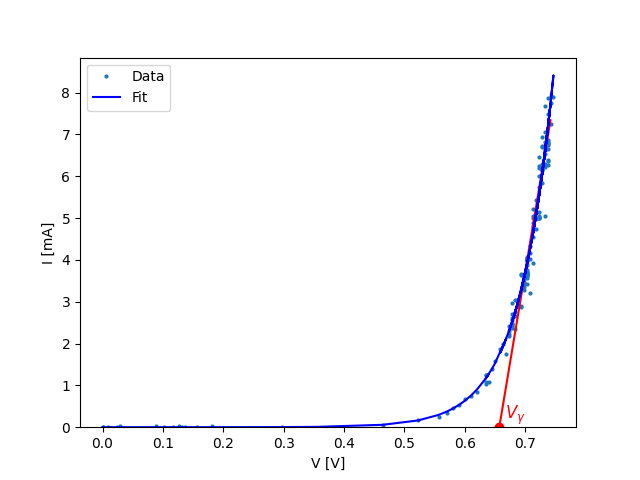
\includegraphics[width=\textwidth]{diodo 1N.png}
		\caption{Diodo 1N4150}
		\label{Plot 1N4150}
	\end{subfigure}
	\begin{subfigure}{0.32\textwidth}
		\includegraphics[width=\textwidth]{plot diodo LED.png}
		\caption{Diodo LED}
		\label{Plot diodo LED}
	\end{subfigure}
	\begin{subfigure}{0.32\textwidth}
		\centering
		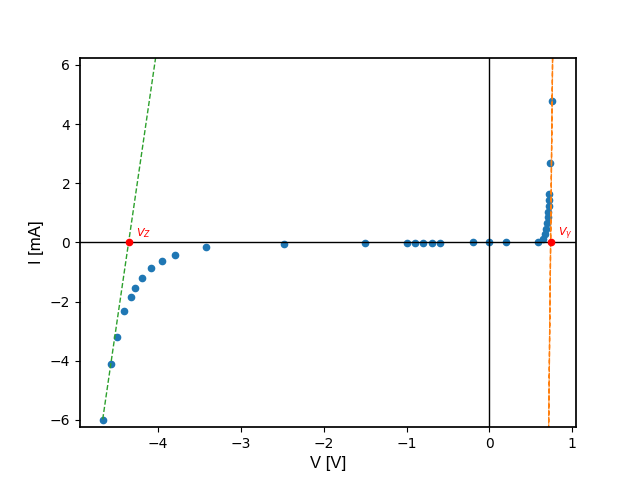
\includegraphics[width=\textwidth]{Caratteristica zener.png}
		\caption{Diodo Zener}
		\label{Zener}
	\end{subfigure}
	\caption{Caratteristica I-V di alcuni Diodi}
	\label{I-V diodi}
\end{figure}
\subsection{3.2 Diodo come raddrizzatore}
\begin{figure}[h!]
	\centering
	\begin{subfigure}{0.475\textwidth}
		\centering
		\begin{circuitikz}[scale=0.7,american, voltage shift=0.5]
			\ctikzset{bipoles/oscope/waveform=sin}
			\draw
			(0,0)to [R,l_=$R$] (4,0)
			to [D,v=$V_d$](4,-3)
			to [short,-](0,-3)
			(0,0) to [oscope,v_=$V_g$](0,-3)
			(4,0) to [short,-](6,0)
			to [rmeterwa,t=V](6,-3)
			to [short,-](4,-3);
		\end{circuitikz}
		\caption{Senza $V_{DC}$}
		\label{Senza VDC}
	\end{subfigure}
	\hfill
	\begin{subfigure}{0.475\textwidth}
		\centering
		\begin{circuitikz}[scale=0.7,american, voltage shift=0.5]
			\ctikzset{bipoles/oscope/waveform=sin}
			\draw
			(0,0)to [R,l_=$R$] (4,0)
			to [D,v^=$V_d$](4,-2)
			to [battery2](4,-3)
			to [short,-](0,-3)
			(0,0) to [oscope,v_=$V_g$](0,-3)
			(4,0) to [short,-](6,0)
			to [rmeterwa,t=V,v^=$V_{out}$](6,-3)
			to [short,-](4,-3);
		\end{circuitikz}
		\caption{Con $V_{DC}$}
		\label{Con VDC}
	\end{subfigure}
	\caption{Circuito raddrizzatore con e senza $V_{DC}$}
	\label{fig: Raddrizzatore}
\end{figure}
Il diodo è un dispositivo che può essere utilizzato come raddrizzatore d'onda, infatti, per la sua caratteristica di far passare correnti in un verso ma non nell'altro permette, ad esempio, di bloccare potenziali negativi. Lo schema circuitale per vedere questo tipo di fenomeno è quello rappresentato in figura \ref{fig: Raddrizzatore}.
\subsubsection{3.2.1 - 3.2.3}
Si è utilizzata una resistenza da $1\unit{\kohm}$ e si è data in ingresso una tensione sinusoidale ad una frequenza $f=1\unit{\kHz}$ con tensione $5V_{pp}$.
Si è poi controllato il voltaggio ai capi di R ed ai capi del diodo.
Il risultato è quello rappresentato in figura \ref{SS}. Come si può notare le tensioni negative sono bloccate dal diodo. Si nota inoltre che la tensione sulla resistenza non raggiunge mai il valore massimo, questa differenza di tensione è proprio dovuta alla caduta di tensione sul diodo.\\
Si è poi ripetuta la misurazione con il diodo in reversed bias ovvero montato nel verso opposto a come mostrato in figura \ref{Senza VDC}. In questo caso il risultato è quello opposto al precedente, vengono pertanto bloccate le tensioni positive come mostra sempre la figura \ref{SS}.
Misure analoghe sono state svolte anche per tensioni di ingresso ad onda triangolare. Chiaramente le considerazioni sono analoghe. Il risultato di tali misure è riportato in figura \ref{TS}.\\
\subsubsection{3.2.4 - 3.2.5}
In quest'attività si è studiato il comportamento del circuito mostrato in figura \ref{Con VDC}.
La differenza quindi con il circuito precedente è la presenza di un generatore di tensione costante a valle del diodo.\\
L'aggiunta di questo generatore di tensione ha portato delle complicazioni sulla misurazione effettiva in laboratorio della tensione ai capi del diodo in quanto sia il generatore di tensione che l'oscilloscopio richiedono il collegamento a massa.\\
Il risultato di tale misura è quello riportato in figura \ref{SC}.
Esattamente come per il circuito precedente si è invertita la polarità del diodo e sono state riprese le misure e si sono quindi ottenuti i risultati riportati sempre in figura \ref{SC}.\\
A differenza del circuito precedente si nota che la tensione di uscita ha registrato uno shift dovuto proprio alla tensione fornita dal generatore a valle del diodo.
\begin{figure}[h!]
	\begin{subfigure}{1\textwidth}
		\begin{minipage}{0.24\textwidth}
			\includegraphics[width=1\textwidth]{Diodo 3.2.(1-2)/V_D_forward.png}
		\end{minipage}
		\hfill
		\begin{minipage}{0.24\textwidth}
			\includegraphics[width=1\textwidth]{Diodo 3.2.(1-2)/V_R_forward.png}
		\end{minipage}
		\hfill
		\begin{minipage}{0.24\textwidth}
			\includegraphics[width=1\textwidth]{Diodo 3.2.(1-2)/V_D_reverse.png}
		\end{minipage}
		\hfill
		\begin{minipage}{0.24\textwidth}
			\includegraphics[width=1\textwidth]{Diodo 3.2.(1-2)/V_R_reverse.png}
		\end{minipage}
		\caption{Tensione ai capi di diodo e resistenza con ingresso un'onda sinusoidale senza $V_{DC}$}
		\label{SS}
	\end{subfigure}
	\hfill
	\begin{subfigure}{1\textwidth}
		\begin{minipage}{0.24\textwidth}
			\includegraphics[width=1\textwidth]{Diodo 3.2.3/Triang_V_D_Forward.png}
		\end{minipage}
		\hfill
		\begin{minipage}{0.24\textwidth}
			\includegraphics[width=1\textwidth]{Diodo 3.2.3/Triang_V_R_Forward.png}
		\end{minipage}
		\begin{minipage}{0.24\textwidth}
			\includegraphics[width=1\textwidth]{Diodo 3.2.3/Triang_V_D_Reverse.png}
		\end{minipage}
		\hfill
		\begin{minipage}{0.24\textwidth}
			\includegraphics[width=1\textwidth]{Diodo 3.2.3/Triang_V_R_Reverse.png}
		\end{minipage}
		\caption{Tensione ai capi di diodo e resistenza con ingresso un'onda triangolare senza $V_{DC}$}
		\label{TS}
	\end{subfigure}
	\hfill
	\begin{subfigure}{1\textwidth}
		\begin{minipage}{0.24\textwidth}
			\includegraphics[width=1\textwidth]{Diodo 3.2.(4-5)/DC_V_D_Reverse.png}
		\end{minipage}
		\hfill
		\begin{minipage}{0.24\textwidth}
			\includegraphics[width=1\textwidth]{Diodo 3.2.(4-5)/DC_V_R_Forward.png}
		\end{minipage}
		\begin{minipage}{0.24\textwidth}
			\centering
			\includegraphics[width=1\textwidth]{Diodo 3.2.(4-5)/DC_V_D_Forward.png}
		\end{minipage}
		\hfill
		\begin{minipage}{0.24\textwidth}
			\centering
			\includegraphics[width=1\textwidth]{Diodo 3.2.(4-5)/DC_V_R_Forward.png}
		\end{minipage}
		\caption{Tensione ai capi di diodo e resistenza con ingresso un'onda sinusoidale con $V_{DC}$}
		\label{SC}
	\end{subfigure}
	\caption{Voltaggio ai capi di diodo e resistenza con una tensione quadrata e triangolare in ingresso con e senza $V_{DC}$}
	\label{Triangular input}
\end{figure}
\newpage

\subsection{3.3 Alimentatore a semionda}
\begin{figure}[h!]
	\centering
	\begin{circuitikz}[american, voltage shift=0.5]
		\ctikzset{bipoles/oscope/waveform=sin}
		\draw
		(0,0)to [D] (4,0)
		to [C](4,-3)
		to [short,-](0,-3)to [oscope,v^<=$V_g$](0,0);
		\draw (4,0) to [short,-](6,0)
		to [R,l=$R_L$,v=$V_L$](6,-3)
		to [short,-](4,-3);
		\draw (6,0) -- (8,0)
		to [rmeterwa,t=V] (8,-3) -- (6,-3);
	\end{circuitikz}
	\caption{Alimentatore a semionda}
	\label{fig: Stabilizzatore}
\end{figure}
In quest'esperienza si verifica il corretto funzionamento di un alimentatore a semionda il cui schema circuitale è quello riportato in figura \ref{fig: Stabilizzatore}. Lo scopo del circuito è quello di raddrizzare una tensione sinusoidale. Per fare ciò si sfrutta il carattere non lineare del diodo e la scarica del condensatore.
\subsubsection{3.3.1}
Lo scopo del circuito è quello di raddrizzare la tensione sinusoidale in ingresso e di mantenere un valore medio di tensione costante.\\
Per farlo si sfrutta il fatto che il diodo non permette il passaggio di corrente in verso opposto e che il condensatore si carica e si scarica in base alla tensione ai suoi capi.\\
In particolare, quando la tensione ai capi del condensatore è minore di quella in uscita dal generatore il diodo si polarizza direttamente e il condensatore si carica,
mentre quando la tensione ai capi del condensatore è maggiore di quella in uscita dal generatore il diodo si polarizza inversamente e il condensatore si scarica.\\
Si è quindi montato il circuito in figura \ref{fig: Stabilizzatore} con $C=10\unit{\nF},R_L=1\unit{\kohm}$, si è variata la frequenza del generatore ($1\unit{\Hz},10\unit{Hz},100\unit{\Hz}$) e si è misurata la tensione ai capi del carico.\\
Il risultato è quello riportato in figura \ref{ripple semi}.\\
Come si nota all'aumentare della frequenza la tensione viene stabilizzata in maniera più efficace. Infatti aumentando la frequenza non si dà il tempo al condensatore di scaricarsi e quindi viene mantenuta una tensione pressoché costante. E' tuttavia importante notare che questo schema di ragionamento (aumentare la frequenza per rendere il valore di tensione più stabile) non può essere portato all'infinito in quanto il condensatore non porterebbe il sistema a riconoscere tensioni dinamiche ed inoltre spesso, nelle configurazioni di utilizzo pratico, non si ha controllo sulla frequenza della tensione in ingresso.
\begin{figure}
	\centering
	\begin{subfigure}{0.32\textwidth}
		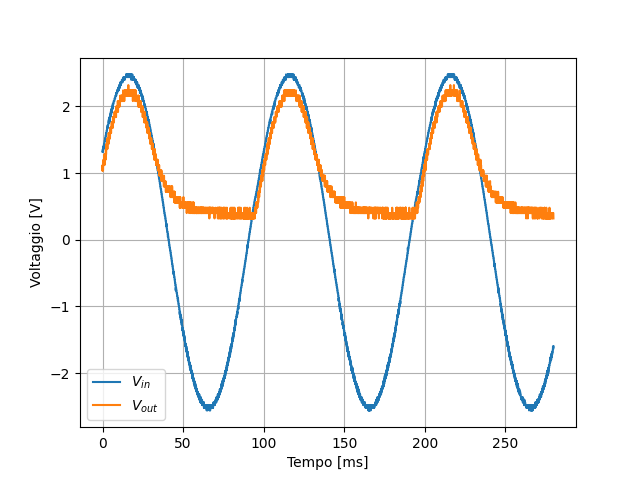
\includegraphics[width=\textwidth]{freq1.png}
		\label{d}
		\caption{\unit{\Hz}}
	\end{subfigure}
	\hfill
	\begin{subfigure}{0.32\textwidth}
		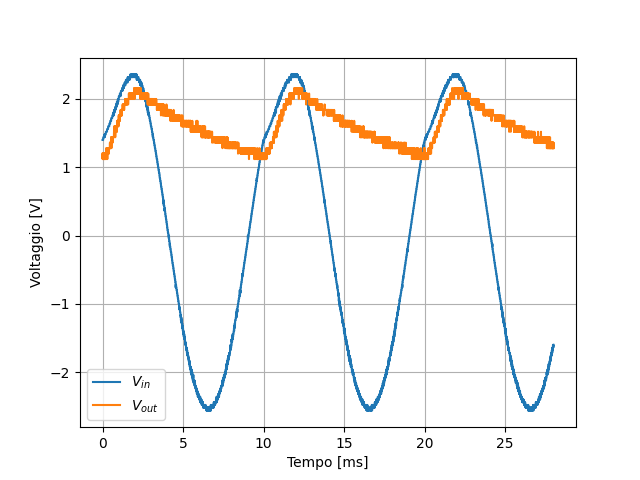
\includegraphics[width=\textwidth]{freq2.png}
		\label{h}
		\caption{100\unit{\Hz}}
	\end{subfigure}
	\hfill
	\begin{subfigure}{0.32\textwidth}
		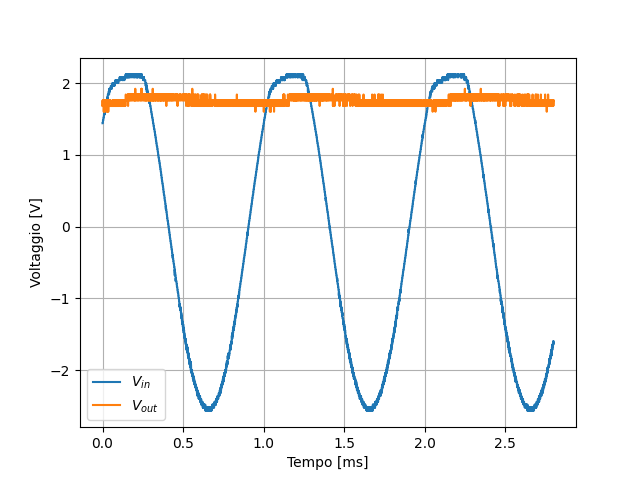
\includegraphics[width=\textwidth]{freq3.png}
		\label{s}
		\caption{1\unit{\kHz}}
	\end{subfigure}
	\caption{Tensione in ingresso ed uscita al variare della frequenza per il circuito stabilizzatore}
	\label{raddr}
\end{figure}
\begin{figure}
	\centering
	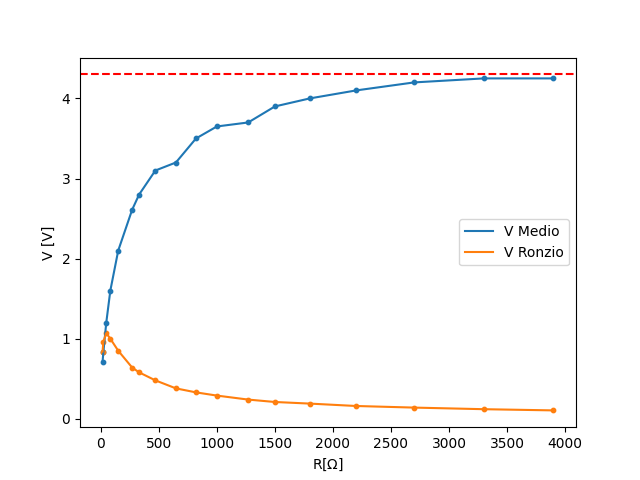
\includegraphics[scale=0.5]{Ripple semionda.png}
	\caption{Tensione media e di ronzio ai capi della resistenza di carico in funzione di quest'ultima}
	\label{ripple semi}
\end{figure}
\begin{subsection}{3.3.2}
	Si è quindi fissata la frequenza ad 1\unit{\kHz} e fatta variare la tensione di carico($R_L$ nel circuito in \ref{fig: Stabilizzatore}). Come si può notare ad alte resistenze di carico la tensione è asintoticamente stabilizzata. A basse resistenze si hanno comportamenti anomali per i quali i valori di ronzio sono relativamente alti e la tensione media decisamente più bassa di quella voluta.
\end{subsection}
\subsection{3.4 Stabilizzatore Zener}
\begin{figure}[H]
	\centering
	\begin{circuitikz}[american, voltage shift=0.5]
		\draw
		(0,0) to [voltage source,v^=$V_g$,invert](0,3)
		to [R,l=$R_z$](4,3)
		to [zzDo,invert](4,0)
		to [short,-](0,0);
		\draw (4,3) to [short,-](6,3)
		to [R,l_=$R_L$,v^=$V_{out}$](6,0)
		to [short,-](4,0);
	\end{circuitikz}
	\caption{Circuito stabilizzatore Zener}
	\label{Stabilizzatore Zener}
\end{figure}
In quest'esperienza si è studiato il comportamento di un alimentatore stabilizzzato realizzato con un diodo Zener.\\
Lo schema circuitale è quello in figura \ref{Stabilizzatore Zener}.\\
Il principio di funzionamento è basato sul fatto che il diodo Zener polarizzato inversamente, una volta raggiunta la tensione di Zener, mantiene costante la tensione ai suoi capi, sfruttando l'effetto Zener.\\
Si è quindi montato il circuito in figura \ref{Stabilizzatore Zener} con $V_g=10\unit{\V}$ alla frequenza di $1\unit{\kHz}$.\\
Per stimare la resistenza $R_z$ si è fatto in modo tale che il diodo Zener non possa dissipare più potenza di quella dissipabile riportata nel datasheet. Si è pertanto andati a controllare la potenza massima dissipabile dal datasheet e si è trovato un valore di $500\unit{\mW}$. Nel caso peggiore ($R_L$ grandi) la corrente viene tutta assorbita dal diodo Zener. Si avrà pertanto:
\begin{equation*}
	I_z=\frac{V_g-V_z}{R_z}
\end{equation*}
Quindi:
\begin{equation*}
	500\unit{\mW}>V_z\cdot I_z \longrightarrow R_z> \frac{V_z(V_g-V_z)}{500}\approx50\unit{\ohm}
\end{equation*}
In linea con l'esigenza di una resistenza maggiore di 50 \unit{\ohm} e con le resistenze disponibili in laboratorio si è scelta una resistenza di 82 \unit{\ohm}.\\
si sono fatte le misure in funzione della tensione di carico $R_L$, il risultato è quello riportato in figura \ref{zenerstab}.\\
Come si può notare, da circa $1\unit{\kohm}$ la tensione viene ben stabilizzata (Ripple relativamente basso) dal circuito alla tensione di Zener.
\begin{figure}[H]
	\centering
	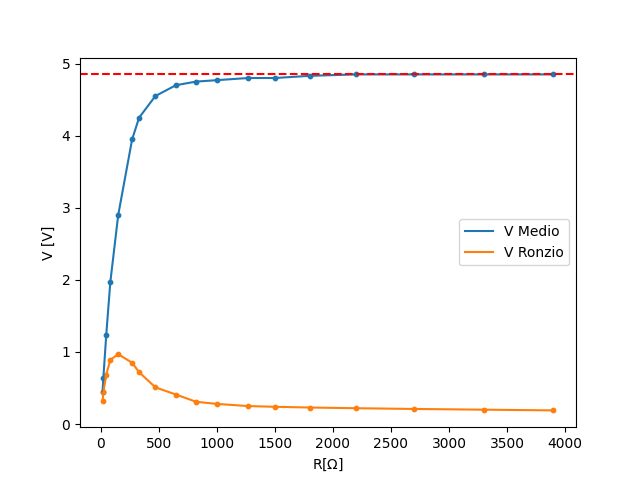
\includegraphics[scale=0.5]{zenerripple.png}
	\caption{Tensione media e di ripple ai capi della resistenza di carico in funzione del valore di quest'ultima}
	\label{zenerstab}
\end{figure}

\subsubsection{3.4 (extra)}
\begin{figure}[h!]
	\centering
	\begin{circuitikz}[american, voltage shift=0.5]
		\draw
		(0,0) to [R,l=$R_g$](2,0)
		to [battery2,v=$V_\gamma$] (4,0)
		to [C](4,-3)
		to [short,-](0,-3)to [voltage source,v=$V_{max}$,invert](0,0);
		\draw (4,0) to [short,-](6,0)
		to [R,l=$R_L$,v=$V_L$](6,-3)
		to [short,-](4,-3);
	\end{circuitikz}
	\caption{Circuito dell'alimentatore a semionda nell'ipotesi di diodo in conduzione}
	\label{diodo in cond}
\end{figure}
Quando si sono misurate le tensioni di ronzio si è notato che per basse resistenze di carico la curva teorica riportata nelle dispense non corrispondeva alle tensioni di ronzio misurate. Questo è un comportamento che ci saremmo dovuti aspettare dato che l'espressione della tensione di ronzio delle dispense è stata trovata per $R_L \xrightarrow{}+\infty$. Tuttavia, nelle misure $R_L\xrightarrow{}0$! Pertanto è necessario riformulare la formula considerando, date le basse resistenze in gioco, anche la resistenza interna del generatore. Un' altro problema è che la tensione massima vista dal carico: per basse resistenze non è più quella erogata dal generatore in quanto a quest'ultima viene tagliato il picco di tensione dal circuito R-Diodo creatosi (L'impedenza della capacità è praticamente nulla ad 1\unit{\kHz}). Per stimare la tensione di ripple supponiamo che la scarica del condensatore avvenga in un periodo, si ha pertanto:
\begin{equation}
	v_C(T)=V_{max}e^{-\frac{T}{\tau}}=V_{max}-\Delta V\Longrightarrow\Delta V=V_{max}\left[ 1-e^{-\frac{T}{\tau}}\right]
	\label{V_ripple}
\end{equation}
Si cerca quindi di stimare $V_{max}$, per fare ciò si considera il diodo in conduzione e la tensione erogata dal generatore massima nell'istante di tempo considerato. Il circuito da analizzare è pertanto quello in figura \ref{diodo in cond} ove si cerca di stimare la tensione ai capi del carico. Per fare ciò si usa Thevenin ai capi di $R_L$.
Per il calcolo della tensione di Thevenin si utilizza il circuito in figura \ref{Vth}.
Si ha quindi:
\begin{equation*}
	V_{max}-V_{\gamma}=R_g I+Z_C I\Longrightarrow I=\frac{V_{max}-V_{\gamma}}{R_g+Z_C}
\end{equation*}
Da cui:
\begin{equation*}
	V_{th}=V_{max} - R_g I - V_{\gamma}\Longrightarrow V_{th}=\frac{Z_C}{Z_C+R_g}(V_{max} - V_{\gamma})
\end{equation*}
Per il calcolo dell'impedenza di Thevenin si utilizza il circuito in figura \ref{Rth}.
\begin{figure}
	\centering
	\begin{subfigure}{0.475\textwidth}
		\begin{circuitikz}[american, voltage shift=0.5]
			\draw
			(0,0) to [R,l=$R_g$](4,0)
			to [C,l=$Z_C$](4,-3)--(0,-3)--(0,0);
			\draw
			(4,0) to [short,-*](5,0)
			to [open](5,-3)
			to [short,*-](4,-3);
		\end{circuitikz}
		\caption{Calcolo $Z_{th}$}
		\label{Rth}
	\end{subfigure}
	\hfill
	\begin{subfigure}{0.475\textwidth}
		\centering
		\begin{circuitikz}[american, voltage shift=0.5]
			\draw
			(0,0) to [R,l=$R_g$](2,0)
			to [battery2,v=$V_\gamma$] (4,0)
			to [C,l_=$Z_C$](4,-3)--(0,-3)
			to [voltage source,v=$V_{max}$,invert](0,0);
			\draw
			(4,0) to [short,-*](5,0)
			to [open,v=$V_{th}$](5,-3)
			to [short,*-](4,-3);
		\end{circuitikz}
		\caption{Calcolo $V_{th}$}
		\label{Vth}
	\end{subfigure}
	\caption{Circuiti per il calcolo dei parametri di Thevenin}
	\label{Thevenin equivalent}
\end{figure}
\begin{figure}
	\centering
	\begin{circuitikz}[american, voltage shift=0.5]
		\draw
		(0,0) to [generic,l=$Z_{th}$](3,0)
		to [R,l=$R_L$](3,-3)--(0,-3)
		to [voltage source,v=$V_{th}$,invert] (0,0);
	\end{circuitikz}
	\caption{Circuito equivalente}
	\label{Circuito equivalente}
\end{figure}
Da cui:
\begin{equation*}
	Z_{th}=\frac{R_gZ_C}{R_g+Z_C}
\end{equation*}
Il circuito equivalente è pertanto quello in figura \ref{Circuito equivalente}
Si trova quindi la tensione ai capi di $R_L$ che risulta essere pari a:
\begin{equation}
	V_L=\frac{R_L}{Z_{th}+R_L}V_{th}
	\label{V_L raddr}
\end{equation}
Se pertanto si inserisce $V_L$ nell'equazione \ref{V_L raddr} all'interno dell'equazione \ref{V_ripple} al posto di $V_{max}$ si ottiene l'equazione:
\begin{equation}
	\Delta V = \frac{R_L}{Z_{th}+R_L}V_{th}\left[ 1-e^{-\frac{T}{\tau}}\right]
	\label{V_ripple_mod}
\end{equation}
Si sono quindi misurati sperimentalmente le tensioni di ronzio tramite l'oscilloscopio e si è confrontato con l'equazione teorica \ref{V_ripple_mod}. Il risultato è quello ottenuto in figura \ref{Figura ripple}.
Come si vede i risultati teorici sono soddisfacenti con i risultati sperimentali ottenuti.
\begin{figure}[h]
	\centering
	\includegraphics[scale=0.5]{Figuraripple.png}
	\caption{Tensione di Ronzio in funzione della resistenza di carico}
	\label{Figura ripple}
\end{figure}